\documentclass[11pt]{article}

\usepackage[margin=1in]{geometry}
\usepackage{graphicx}
\usepackage{booktabs}
\usepackage{caption}
\usepackage{amsmath}
\usepackage{hyperref}
\usepackage{lmodern}
\usepackage{parskip}

\hypersetup{
  colorlinks=true,
  linkcolor=blue!60!black,
  urlcolor=blue!60!black,
  citecolor=blue!60!black
}

\graphicspath{{../results/figures/}}

\title{Financial News Sentiment Analysis for S\&P 500 Return Prediction}
\author{}
\date{}

\begin{document}
\maketitle

\section{Introduction}

This project applies natural language sentiment models to a corpus of Wall Street Journal financial news articles published between 2017 and 2020, and asks whether the resulting sentiment signal can predict the next-day return of the affected S\&P 500 stocks. I compare a zero-shot pretrained FinBERT model against two small neural networks fine-tuned directly on returns, and I backtest each on a simple trading strategy at the end.

The main problem I ran into is that FinBERT can only read 512 tokens at a time. Wall Street Journal articles are often much longer than that, and a naive use of FinBERT silently throws away everything past the first 512 tokens. The simple way to deal with this is to keep only the first 512 tokens of each article, which is not unreasonable since news articles usually put their most important point at the top. But if a later paragraph adds a qualification or changes the tone, that information is lost.

The goal of this report is therefore not to build a model that beats the market. Next-day stock returns are very noisy, and no text model is going to fix that. The goal is to find a more robust way to read long news articles and feed them to a sentiment model. As shown later, I split each article into smaller pieces, train the model on those pieces, and combine the results back together. The details are in the methodology sections.

All code used in this report is available at \url{https://github.com/WillInvest/Sentiment-Analysis-}.

\section{Data}

\subsection{Raw inputs}

The project starts from two files. The first is a news file with about 593{,}000 Wall Street Journal articles published between January 2017 and December 2020. Each article has a publication date, a title, a body, and a string of one or more tagged tickers. The second is a price file with daily closing prices for the S\&P 500 constituents and the index itself. The publication dates in the news file are date-only with no time of day, which means I cannot tell whether an article hit before market open or after the close. This limitation will come back later.

\subsection{Final dataset statistics}

After processing (described in the next two sections), the raw files reduce to a clean training table of about 20{,}550 rows covering 381 unique tickers from January 2017 through December 2020. The mean one-day return is essentially zero and the positive class rate is about 53\%, slightly tilted upward because the period was mostly a bull market. The big drop from 593{,}000 raw articles to 20{,}550 useful rows happens because most Wall Street Journal articles cover politics, world news, or companies outside the S\&P 500, none of which I can match to a stock price.

\subsection{Data exploration}

Before building anything I looked at the data to understand what I was working with. The single most important fact is the article length distribution. I tokenized a sample of 5{,}000 articles with FinBERT's tokenizer to see how long they actually are in tokens, since tokens are the unit FinBERT cares about, not words.

\begin{figure}[ht]
\centering
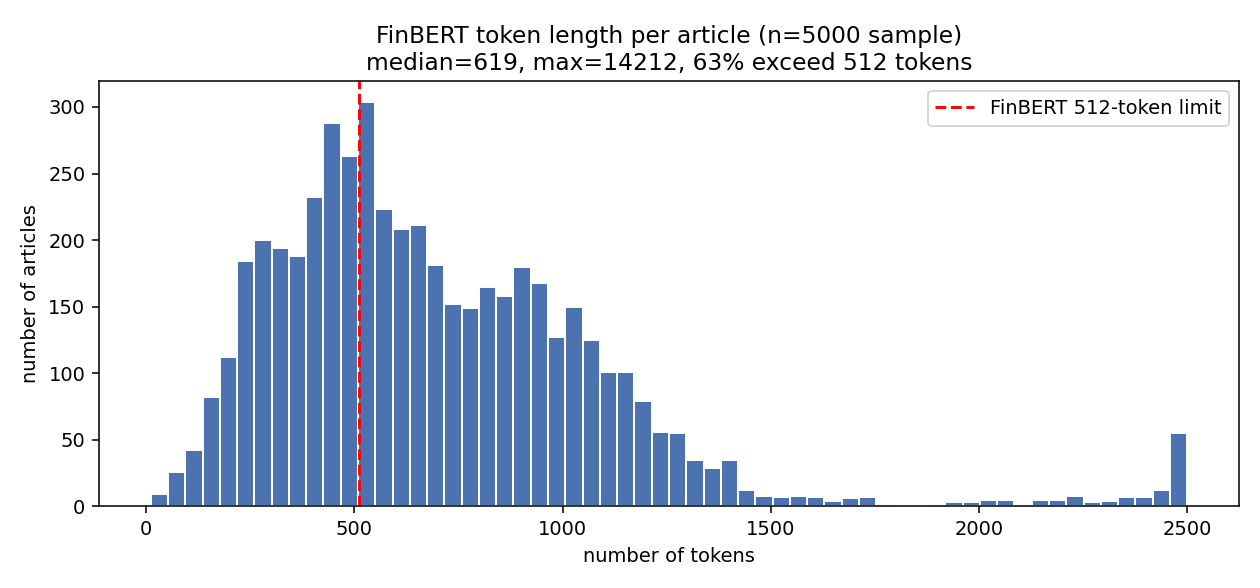
\includegraphics[width=\textwidth]{eda_token_length.png}
\caption{Distribution of article lengths in FinBERT tokens. The dashed red line is FinBERT's 512-token hard limit. About 63\% of articles in the dataset exceed it, with the median article at 619 tokens and the longest at over 14{,}000.}
\label{fig:token_length}
\end{figure}

The median article is 619 tokens, the mean is 712 tokens, and the longest article in the sample is over 14{,}000 tokens. About 63\% of the articles in the dataset are longer than 512 tokens, which means almost two thirds of the articles cannot fit into FinBERT in one piece. A naive head-only approach throws away the body of nearly every long article. This is the gap that the chunking method in the next section fills.

Coverage over time is roughly even with around 400 to 500 articles per month, so the rolling time windows I use later all have comparable test set sizes. The dataset is concentrated on mega-cap stocks, with Amazon at the top with about 1{,}333 articles and the rest of the top twenty filled by other large-cap names. The long tail of 381 tickers each have only a few articles, so the model is mostly learning what the Wall Street Journal says about big technology companies.

\section{From raw files to a clean dataset}

This section walks through how the two raw files become one row per article, with a return label attached. Real example values from the actual data are used so the steps are easy to follow.

The first step is matching every article to a price. Some articles cover companies that are not in the stock list because they are foreign, private, or simply not S\&P 500 constituents. For those I cannot compute a return, so I drop them. This is by far the biggest filter, removing about 97\% of the raw articles and leaving me with roughly 20{,}550 articles, each tagged with a single ticker I have prices for.

The second step is shifting weekend and holiday articles to the next trading day. The market is closed on those days, so an article published then has no same-day price. I push the date forward to the next trading day, which is the first day the market could actually react to the news. As a real example, an article titled ``Retailers Face Hit Under Tax Plan'' tagged WMT was published on Saturday January 7, 2017. Saturday and Sunday are both not trading days, so I look forward to Monday January 9, which is a trading day, and use that as the article's date. The original date is kept in a separate column for auditing. About 3{,}173 of the 20{,}550 rows, or roughly 15\% of the dataset, get shifted in this way.

The third step is computing the next-day return. For each ticker and date pair I look up the closing price on that day and on the next trading day. The return is just the percentage change between the two. Continuing the example above, WMT closed at \$67.18 on Monday January 9 and \$66.71 on Tuesday January 10, giving a return of $-0.0070$ or about $-0.7\%$. So the article's label is $r_{1d} = -0.0070$. Articles where the next-day price is not available, such as articles published on the very last day of the dataset, are dropped.

After these three steps I have 20{,}550 rows. Each row contains an article identifier, a ticker, the trading date, the original publication date, the article text, and the next-day return. This clean dataset is the input to everything that follows.

\section{From clean dataset to model-ready features}

This section turns each article's text into the numbers the model will see. There are three sub-steps, split, score, and combine, followed by a final time-based train and test split.

\subsection{Splitting articles into chunks}

FinBERT can only read 512 tokens at a time, which is roughly 350 words. Most Wall Street Journal articles in the dataset are longer than this, so I have to break them into smaller pieces called chunks.

I split by sentence, never in the middle of one. Cutting a sentence in half loses meaning, since a phrase like ``the outlook is not good'' can flip from negative to positive if the word ``not'' gets cut off. Once I have the sentences, I pack as many as I can into a single chunk without going over 510 tokens, leaving 2 tokens for the special start and end markers FinBERT adds. When I start the next chunk, I go back two sentences from where the previous one ended, so neighboring chunks share a small overlap and the context at the boundary is not lost. In the dataset the average article makes about 2 chunks, and around 36\% of articles need 2 or more chunks. The total number of chunks across the dataset is 40{,}755.

To check whether all this extra work is actually buying me anything, I compared the score from the sliding-window approach with the score from the naive head-only approach. The figure below shows the comparison on the 13{,}121 articles that needed two or more chunks, which are the only ones where the two approaches can disagree.

\begin{figure}[ht]
\centering
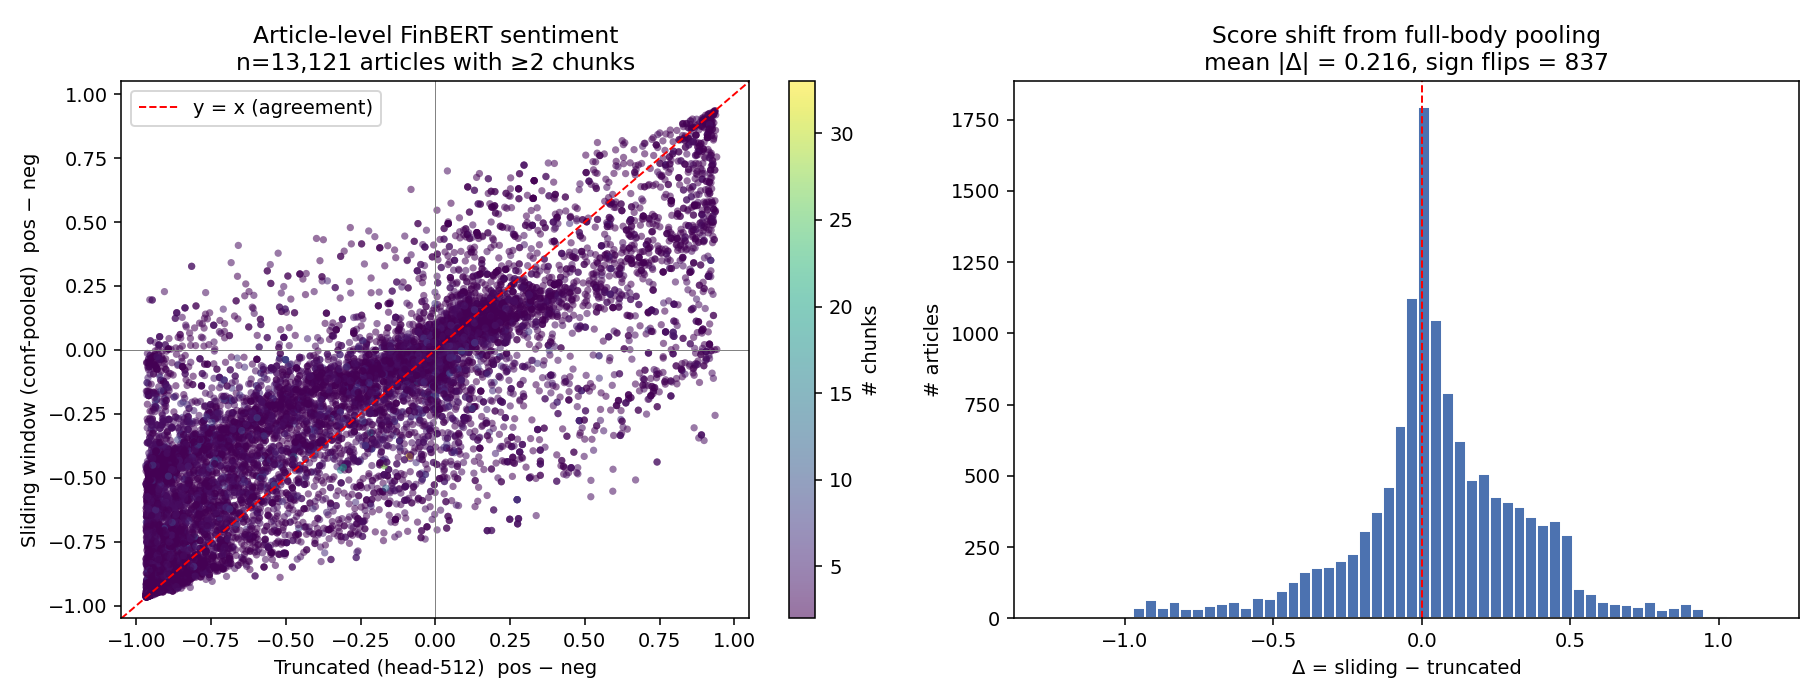
\includegraphics[width=\textwidth]{sentiment_ablation.png}
\caption{Sliding-window pooled score versus naive head-only truncation, restricted to articles with two or more chunks. The left panel is a per-article scatter; the red dashed line marks perfect agreement. The right panel shows the distribution of the difference between the two methods. The mean absolute change is 0.216 and the two methods disagree on the sign of the sentiment for 837 articles.}
\label{fig:ablation}
\end{figure}

The left panel is a scatter where each dot is one article, with the naive truncation score on the x-axis and the sliding-window score on the y-axis. If the two methods always agreed, every point would sit on the red dashed diagonal. They mostly do agree on extreme cases where the article is very positive or very negative, but in the middle there is a wide cloud. These are the articles where reading the full body changes the sentiment compared to reading only the lead. The right panel shows the distribution of the difference between the two methods. The mean absolute change is 0.216, and on 837 articles the two approaches disagree on whether the article is positive or negative. That is a non-trivial chunk of the dataset where a head-only score gets the verdict wrong.

\subsection{Scoring each chunk with FinBERT}

Every chunk goes through FinBERT and comes back with four numbers. Three of them are FinBERT's sentiment probabilities for positive, negative, and neutral, each between 0 and 1. The fourth is the highest of those three, which I call the chunk's confidence and which tells me how sure FinBERT is about its answer. On top of these I also save the chunk's representation vector from FinBERT's last hidden layer, a 768-number vector. This is the rich feature the model will actually train on; the three sentiment probabilities are extra hints sitting alongside it.

As a concrete example, one article in the dataset has three chunks. The first chunk is mildly positive with positive 0.570, negative 0.017, neutral 0.413, so the confidence is 0.570 and FinBERT is only somewhat sure. The second chunk is strongly neutral with positive 0.073, negative 0.025, neutral 0.902, so the confidence is 0.902. The third chunk is also strongly neutral at 0.913 confidence. Chunks two and three are very confident; chunk one is uncertain.

\subsection{Combining chunks with confidence weights}

Now I have three chunks but I want one number for the whole article. The intuition is simple: chunks where FinBERT is more sure should count more.

For each chunk I use its confidence as a weight, then normalize so the weights add up to one. For the example above, the total confidence across the three chunks is $0.570 + 0.902 + 0.913 = 2.385$. The first chunk's weight is $0.570 / 2.385 = 0.239$, the second is $0.378$, and the third is $0.383$. I then multiply each chunk's number by its weight and add them up. The two high-confidence neutral chunks take 76\% of the total weight, so the article's overall score is roughly neutral, even though the first chunk leaned positive on its own. This matches what a human reader would conclude. The same idea works for the trained model: instead of combining FinBERT's probabilities, the model produces one number per chunk, and I combine those numbers using the same confidence weights.

\subsection{Splitting into rolling time windows}

Finally I split the dataset into training, validation, and test sets by time, not randomly. Random splits would let the model see the future during training, which is cheating. I use three rolling windows. Each window has 24 months of training, 6 months of validation, and 6 months of testing, and they slide forward by 6 months. I leave a 3-day gap between train and validation and between validation and test so a next-day return cannot accidentally appear on both sides of the cut. The first window trains on 2017--2018 and tests on the second half of 2019; the second trains on the second half of 2017 through the first half of 2019 and tests on the first half of 2020; the third trains on 2018--2019 and tests on the second half of 2020.

\section{Evaluation}

\subsection{The three models being compared}

I compare three models, all using the same chunked features and the same confidence-weighted aggregation. The first is the pretrained baseline, which is just zero-shot FinBERT with no training on returns. I collapse its three sentiment probabilities into a single scalar by computing positive minus negative, and I threshold at zero for binary up or down predictions. The second is a fine-tuned regressor, a small neural network trained with mean squared error loss to predict the continuous next-day return. The third is a fine-tuned classifier trained with binary cross-entropy loss to predict whether the next day's return is positive.

The two fine-tuned models are small multilayer perceptrons that take a 771-dimensional input, made up of FinBERT's 768-dimensional representation vector plus the three sentiment probabilities, and output a single number per chunk. The default architecture has two hidden layers of size 64 and 32 with ReLU activations and dropout of 0.2. Training uses the Adam optimizer with a learning rate of $10^{-3}$ and a batch size of 64 articles, for up to 100 epochs with early stopping on the validation loss.

\subsection{Combining chunks inside the model: padding, mask, and weights}

Because different articles produce different numbers of chunks, the model has to handle a variable number of inputs per article during training. A deep learning model expects a rectangular block of numbers, not a ragged one, so I need a trick to turn a batch of articles with varying chunk counts into something the network can consume. This is where padding comes in.

Suppose a training batch has three articles, the first with two chunks, the second with five, and the third with three. The width of the batch is set to the longest article's chunk count, which is five. The first article is then padded with three slots of zeros so it looks like a five-chunk article, and the third article is padded with two slots. The result is a rectangular tensor where every article has exactly five slots, some of them real and some of them zero-padding. This is what the model sees at its input layer.

The problem with padding is that the zero slots are not real chunks and should not contribute to the article's prediction. If the model simply averaged over all five slots, the pretend zero chunks would dilute the real ones. To prevent this, I carry a second tensor of the same shape called the mask, where a value of 1 marks a real chunk and a value of 0 marks padding. Before the aggregation step, I multiply the per-chunk predictions by the mask, which zeros out anything the model produced for a padded slot. The mask is cheap to build and makes the padding invisible to the downstream computation.

The confidence weights enter at the same stage. Each real chunk has its own weight, computed from its FinBERT confidence exactly as described in section 4, and the weights for a given article are normalized so they add up to one across the real chunks only. Padded slots get weight zero. The model's article-level prediction is then the sum over all slots of (per-chunk prediction) times (mask) times (weight). Because the padded slots have both a mask of zero and a weight of zero, they contribute nothing to the final sum, which is exactly what I want. The weighted sum lands on a single number per article, and the loss function compares that number against the article's return label.

The reason I do the aggregation inside the model instead of computing the per-chunk predictions first and then combining them in a separate step is that it guarantees the training loop and the evaluation loop use exactly the same function to collapse chunks. There is no risk of training with one aggregation rule and evaluating with another, because there is only one function and it sits inside the forward pass.

\subsection{Metrics and default-configuration results}

The project specification asks for both regression and binary classification metrics. For the regressor I report mean squared error and $R^2$ against the actual next-day return. For binary metrics I threshold each model's score at zero (or 0.5 for the classifier sigmoid output) and compute accuracy and F1 against the sign of the actual return. The fine-tuned regressor is therefore evaluated twice from the same prediction column, once as a continuous output and once as a thresholded output. Only one regression model is trained, in line with the spec.

The default configuration produces these test set numbers:

\begin{table}[h]
\centering
\small
\begin{tabular}{llrrrrr}
\toprule
Window & Model & $n$ & MSE & $R^2$ & Acc & F1 \\
\midrule
w1 & regressor  & 2569 & $6.26{\times}10^{-4}$ & $+0.0004$ & 0.521 & 0.671 \\
w1 & classifier & 2569 & --- & --- & 0.505 & 0.603 \\
w1 & baseline   & 2569 & --- & --- & 0.494 & 0.390 \\
w2 & regressor  & 2342 & $1.93{\times}10^{-3}$ & $-0.002$ & 0.521 & 0.685 \\
w2 & classifier & 2342 & --- & --- & 0.521 & 0.671 \\
w2 & baseline   & 2342 & --- & --- & 0.473 & 0.313 \\
w3 & regressor  & 2499 & $5.32{\times}10^{-4}$ & $-0.004$ & 0.497 & 0.664 \\
w3 & classifier & 2499 & --- & --- & 0.490 & 0.625 \\
w3 & baseline   & 2499 & --- & --- & 0.496 & 0.393 \\
\bottomrule
\end{tabular}
\caption{Test-set metrics for the three models on each rolling window using the default architecture.}
\label{tab:default_results}
\end{table}

The $R^2$ values are essentially zero across all three windows. Predicting daily stock returns from text alone is genuinely hard. Accuracy hovers between 49\% and 52\%, just slightly above chance, and the trained models beat the baseline on accuracy in four of the six cases by margins of two to five percentage points. The F1 scores look high at around 0.62 to 0.69 for the trained models, but this is partly a consequence of the data being positive-skewed: the trained models lean toward predicting up, which inflates recall on the majority class. The baseline's lower F1 of about 0.39 reflects FinBERT's bearish bias on financial news rather than poor calibration.

\subsection{Hyperparameter sweep}

I swept three knobs that the project specification calls out: the number of hidden layers (1, 2, or 3), the hidden width (32, 64, or 128, uniform across layers), and the activation function (ReLU, GELU, or LeakyReLU). The full grid is 27 configurations, and each is trained on every rolling window for a total of 81 runs. All training uses the regressor head with mean squared error loss.

\begin{figure}[ht]
\centering
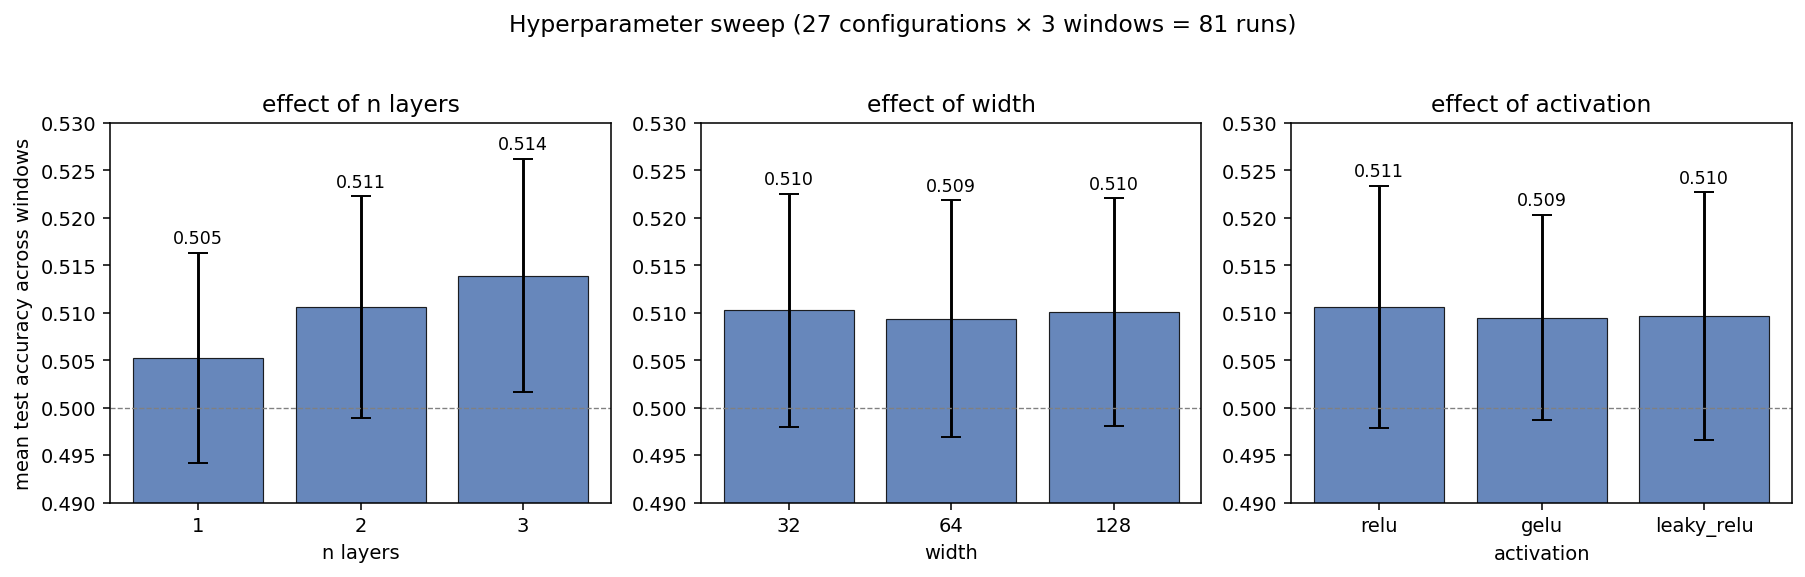
\includegraphics[width=\textwidth]{hp_sweep_marginals.png}
\caption{Marginal effect of each hyperparameter on mean test accuracy across the three rolling windows. Bars show the average over all configurations that share the given value, with error bars showing the standard deviation. The dashed grey line at 0.5 marks chance accuracy.}
\label{fig:sweep}
\end{figure}

The figure above shows the marginal effect of each knob averaged over the others. Three things stand out. First, depth helps slightly: going from one to three hidden layers buys about 0.5 percentage points each step, a small but monotonic improvement. Second, width is essentially irrelevant: the three width settings are within 0.001 of each other on accuracy, suggesting that with roughly 14{,}000 training rows the model is not capacity-limited at any of these widths. Third, the activation function barely matters; ReLU edges the others by 0.001, well within sampling noise. GELU is the most stable across windows in terms of standard deviation, which makes it a reasonable default if minimum variance is the goal.

The best single configuration in the full grid is three layers, width 128, with GELU activation, achieving a mean test accuracy of 0.5202 across the three rolling windows. This is about 1 percentage point better than the default, and about 3.2 percentage points better than the zero-shot FinBERT baseline. None of the 81 configurations produces a meaningful $R^2$ on the regression task. The model is winning small margins on the binary task by adapting to the class prior, not by learning a strong predictive map. This matches the pattern I would expect: architecture choices move accuracy by one or two percentage points, while the structural choices (sliding-window pooling, chunk-based aggregation, frozen FinBERT features) and the data limitations (date-only timestamps, daily horizon) set the ceiling.

\section{Sentiment versus market trend}

So far I have looked at sentiment as a per-article, per-day signal. The project specification also asks me to step back and look at the bigger picture. Do months with more positive news come before months with higher S\&P 500 returns? To answer this, I average each article's sentiment by month and compare each month's average sentiment with the next month's S\&P 500 return. This is a coarser and more forgiving timescale than daily prediction.

For the pretrained baseline I use the confidence-weighted positive-minus-negative score for every article, averaged by publication month. For the fine-tuned regressor I use the predicted next-day return, also averaged by month. I then run a linear regression of next-month S\&P 500 return on monthly sentiment. The pretrained baseline is reported on two periods: the full 4-year range (47 months) to see the long-run relationship, and the 18-month head-to-head window from July 2019 to December 2020 where the fine-tuned model also has out-of-sample predictions, so the two models can be compared directly.

\begin{table}[h]
\centering
\small
\begin{tabular}{llrrrr}
\toprule
Model & Period & Months & Slope & $R^2$ & Correlation \\
\midrule
Pretrained          & 2017-02 to 2020-12 (full)          & 47 & $-0.136$ & 0.043 & $-0.207$ \\
Pretrained          & 2019-07 to 2020-12 (head-to-head)  & 18 & $-0.285$ & 0.163 & $-0.404$ \\
Fine-tuned regressor & 2019-07 to 2020-12 (head-to-head) & 18 & $-3.99$  & 0.003 & $-0.055$ \\
\bottomrule
\end{tabular}
\caption{Linear regression of next-month S\&P 500 return on monthly sentiment. The pretrained model has two rows: the full 4-year window, and the 18-month head-to-head window that overlaps with the fine-tuned model's out-of-sample period.}
\label{tab:market_trend}
\end{table}

The most surprising result is that the pretrained relationship is negative, not positive. Months with higher pretrained sentiment are followed by lower S\&P 500 returns on average. On the full 4-year window this shows up as a modest correlation of $-0.21$ with an $R^2$ of about 4\%, and on the narrower 18-month window it strengthens to $-0.40$ with an $R^2$ of about 16\%. This is the opposite of the naive intuition that positive news leads to a positive market, but it is consistent with a finance idea called sentiment reversal or mean reversion. When news is unusually positive, investors have likely already bought, and the next month sees a pullback. When news is unusually negative, like the early-COVID weeks of March 2020, the market tends to recover. The 18-month window happens to include exactly that crash-and-rebound period, which is part of why the negative correlation looks stronger there than over the full 4 years.

The fine-tuned regressor, in contrast, is essentially uncorrelated with the next-month S\&P 500 return. This is also a meaningful finding, but it points in a different direction. The fine-tuned model was trained to predict individual stock returns one day ahead, not market-wide direction one month ahead. It learned a signal that happens to lose its market-trend alignment when aggregated up to a coarser time scale. The model is good at the narrow task it was trained on and bad at the broader task it was never asked to do, which is fair behavior, not a bug.

A few caveats are worth keeping in mind. The 18-month window is small and dominated by one extreme event, the COVID crash and recovery, so the $-0.40$ correlation should not be taken as a stable estimate of the long-run relationship. Also, the comparison is not perfectly apples-to-apples in scale: the pretrained score lives on a $[-1, 1]$ sentiment scale, while the fine-tuned score lives on the scale of daily returns of about $\pm 0.01$, so the slopes are not directly comparable. Only the correlations and $R^2$ values can be compared across the two models.

\section{Trading strategies}

The previous sections measured the model on prediction metrics. A more concrete question is whether trading on these signals would actually make money. This section runs three simple backtests on the same 18-month out-of-sample window and compares them to a buy-and-hold of the S\&P 500.

All three strategies use the same trade rules so the comparison is fair. When a signal triggers on a given day, I open the position at that day's close. I hold for at most 5 trading days. Each day I check the cumulative return: if it reaches $+3\%$ I take profit, if it falls to $-2\%$ I cut the loss, and if neither happens by day 5 I close at that day's close. All positions are equal-weighted, there is no leverage, and I ignore transaction costs and slippage. This is intentionally simple; a richer backtest with realistic costs and position sizing is out of scope for this report.

The three strategies differ only in which signals they trade. The first is the pretrained baseline as a long-only strategy, which buys whenever the confidence-weighted FinBERT sentiment score is positive, that is, whenever zero-shot FinBERT thinks the article is bullish. The second is the fine-tuned regressor as a long-only strategy, which buys whenever the trained model's predicted next-day return is positive. The third is the fine-tuned regressor as a long-short strategy, which buys when the prediction is positive and short-sells when the prediction is negative. The third strategy is the only one that uses the full distribution of model outputs instead of a one-sided filter.

\begin{figure}[ht]
\centering
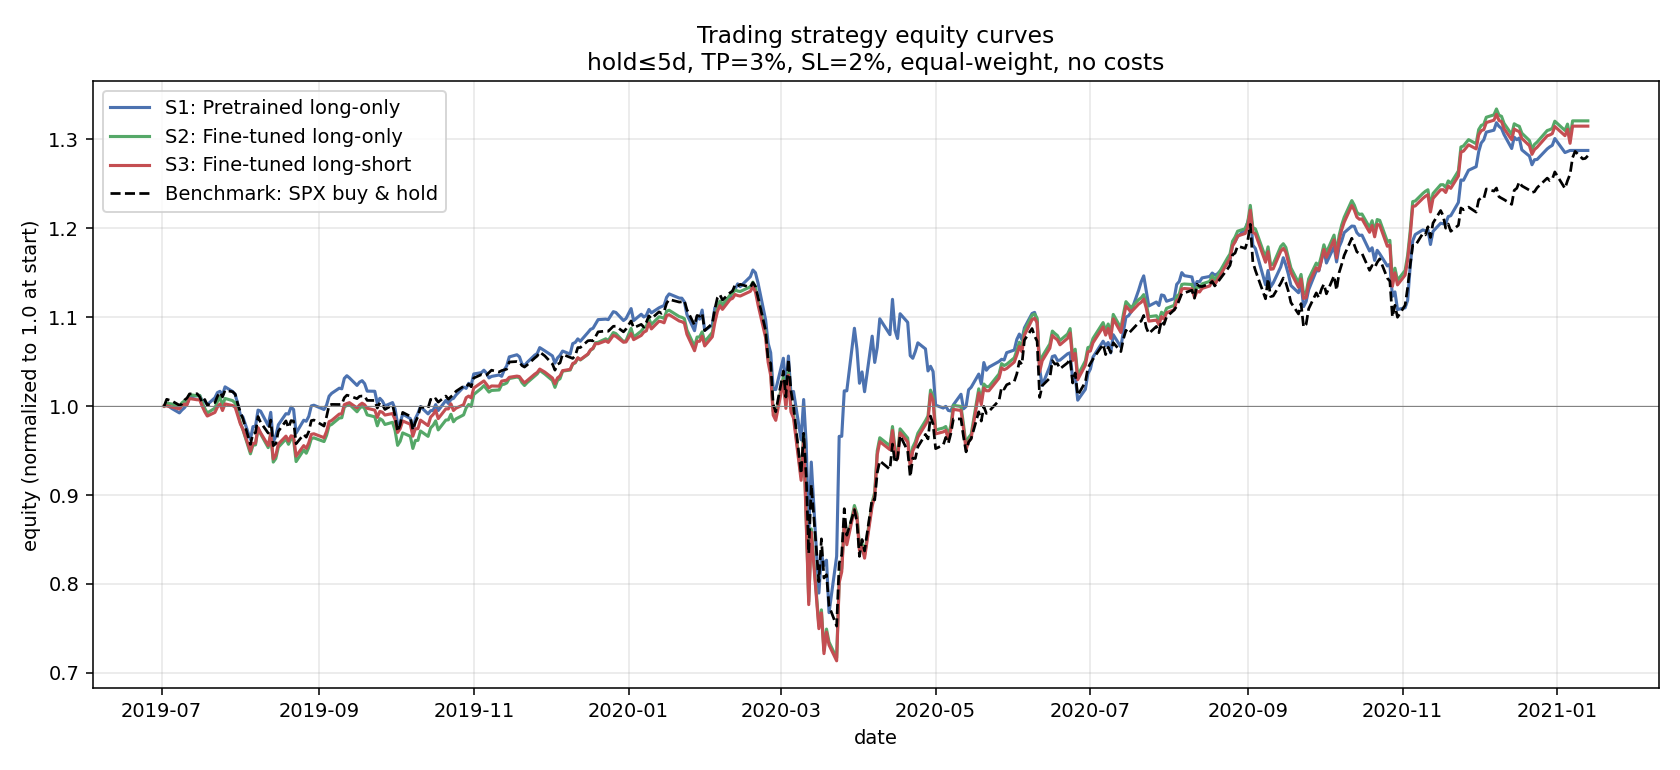
\includegraphics[width=\textwidth]{trading_pnl.png}
\caption{Equity curves for the three trading strategies and the S\&P 500 buy-and-hold benchmark, normalized to 1.0 at the start of the test period. All three strategies use a 5-day maximum holding period, a $+3\%$ take-profit, and a $-2\%$ stop-loss, and are run on the same 18-month out-of-sample window.}
\label{fig:pnl}
\end{figure}

\begin{table}[h]
\centering
\small
\begin{tabular}{lrrrrrr}
\toprule
Strategy & Trades & Win rate & Total return & Annualized & Sharpe & Max drawdown \\
\midrule
Pretrained long-only      & 2189 & 49.0\% & 28.8\% & 17.8\% & 0.67 & $-33.4\%$ \\
Fine-tuned long-only      & 7227 & 50.2\% & 32.1\% & 19.8\% & 0.74 & $-37.1\%$ \\
Fine-tuned long-short     & 7410 & 50.1\% & 31.5\% & 19.5\% & 0.73 & $-37.1\%$ \\
S\&P 500 buy and hold     &    1 & ---    & 28.2\% & 17.5\% & 0.71 & $-33.9\%$ \\
\bottomrule
\end{tabular}
\caption{Backtest statistics for the three strategies and the benchmark over the 18-month out-of-sample window from July 2019 to January 2021.}
\label{tab:trading}
\end{table}

The honest reading of the results is that all three strategies roughly match the S\&P 500 benchmark and none of them generate clear alpha. The fine-tuned long-only strategy edges the benchmark by about 4 percentage points on total return and 0.03 on Sharpe ratio, which is small enough to be inside sampling noise on an 18-month window. The pretrained long-only strategy actually underperforms the index slightly on Sharpe at 0.67 versus 0.71. The long-short version of the fine-tuned model adds nothing over its long-only sibling, which makes sense given how rarely the model produces strongly negative predictions.

The win rates tell a related story: all three strategies hover right around 50\%, just like the per-day accuracy numbers in the previous section. The model is tilted slightly toward up in a market that mostly went up over this period, so the strategies inherit the market's drift rather than adding skill on top of it. The COVID crash in early 2020 also pulls the maximum drawdown of all four lines down to roughly $-34\%$ to $-37\%$, which says the strategies are not meaningfully hedged against systematic risk. That said, matching the index without losing money is not nothing. The fine-tuned long-only strategy makes 7{,}227 small bets across 18 months, takes occasional profits at $+3\%$ and cuts occasional losses at $-2\%$, and ends up roughly where the index ends up. It is a live demonstration that the model's signal is at least not destructive. Whether it adds real alpha would need a much longer evaluation window, transaction costs, and a more careful position-sizing rule before I would be willing to claim it.

\section{Discussion and use of AI}

The sentence-aware sliding window with confidence-weighted pooling recovered information from the 63\% of articles longer than 512 tokens, but the daily return signal itself stayed near zero across all 81 hyperparameter configurations and the trading strategies essentially matched the S\&P 500 benchmark. Limits include date-only timestamps, mega-cap concentration, the frozen encoder, and the short test window.

I used the superpowers brainstorming plugin inside Claude Code as a thinking partner early on. I told it the biggest concern I had was FinBERT's 512-token context window, and we went back and forth through several design iterations before landing on the final architecture. An intermediate plan I considered was to treat each chunk as a fully independent training row and train the model on them separately, then join the per-chunk predictions back together at evaluation time. That approach had a clear problem: longer articles produce more chunks, so longer articles would get more weight during training just because they were split into more pieces. I considered patching this with a $1/n$ re-weighting on the loss, but eventually I decided it was cleaner to change the model architecture instead, moving to a three-dimensional batch layout (articles by chunks by features) with padding and masks, so that each article-ticker pair contributes exactly one loss term no matter how many chunks it produced. From there Claude Code helped me refine the implementation for more efficient parallel execution on the GPU, and caught several bugs in my trading backtest and evaluation code along the way.

\end{document}
